\chapter{Langlands 对应}\label{ch:13}

\begin{keytakeaways}
本章把几何 Langlands 纲领翻译为算术语言。物理图像是四维规范理论 $\cA_G$ 与它的电磁对偶 $\cB_{G^\vee}$：把三维流形换成函数域或数域，把纽结换成素点，则’t~Hooft 线算子（在 $G$ 一侧由 $\Rep(G^\vee)$ 标号）应被 Wilson 线算子（在 $G^\vee$ 一侧由局部系统标号）实现。由此得到非分歧 Langlands 对应的谱分解猜想：自守形式层沿 $\Loc_{G^\vee}(C)$ 分解，且应为对偶层 $\omega$。分歧情形需要引入局部 Langlands 对应——它正是“某条特定曲线上的几何 Langlands”，在导出意义下表现为平滑表示范畴与 $\QC(\Loc_{G^\vee})$ 之间的等价（或其全子范畴），而 $L$-函数是把两侧的数值数据（Hecke 特征值与 Frobenius 特征值）粘合起来的“神奇胶水”。
\end{keytakeaways}

\section{几何 Satake}\label{sec:13-1}

\begin{flushright}\small 第 31 讲；2021 年 6 月 3 日\end{flushright}

\begin{sectionkey}
本节的核心是：几何 Satake 就是“线算子”版本的对偶性——这个“自守 TFT”中 $S^2$ 上的线算子所成的范畴，同构于 Langlands 对偶群的表示；而把它降到 $S^2\times S^1$ 上做范畴化/去范畴化，就得到表示环 $|\Rep(G^\vee)|$。
\end{sectionkey}

回忆我们可以用这个“自守 TFT”中的线算子，也就是赋值 $\cA_G(S^2)$，来表述几何 Satake。于是几何 Satake 说，它可以与 Langlands 对偶的表示等同起来：
\begin{equation}\tag{13.1}
\left(\cA_G(S^2),*\right)\simeq \Rep(G^\vee).
\end{equation}

事实上，这正是我们对 $G^\vee$ 的定义。回忆一下，从物理上看，$\cA_G(S^2)$ 由 't~Hooft 线算子构成，所以它们是这个四维规范场论的一维缺陷。它们是 Dirac 单极子的一种推广。我们在电磁学中见过这些：四维中有一条单极子的世界线，而规范场被允许在其上有奇点。所以，如果我们有四维中的一条线，其链环是一个二维球面，而在 $S^2$ 上给定一个丛、或者更确切地说给定它的 Chern 类，就是在给定单极子本身的电荷。

在交换情形，电荷是一个整数，但现在电荷是表示环 $|\Rep(G^\vee)|$ 中的一个元素。还有更具体的东西，类似于交换情形中所见的，那就是 't~Hooft 圈算子。给定四维流形中的一个圈，它的链环现在是 $S^2\times S^1$，于是 $\cA_G(S^2\times S^1)$ 的元素就是圈的可能的“标号”。由我们关于范畴化的讨论，现在我们知道：
\begin{align}
\cA_G(S^2\times S^1)&=\dim\cA_G(S^2) \tag{13.2}\\
&=|\Rep(G^\vee)|. \tag{13.3}
\end{align}
所以，经典地看，'t~Hooft 单极子是放在四维中一个闭圈上的东西，用一个对偶群 $G^\vee$ 的表示来标记；但现在它只是一个由表示构成的向量空间。
% [Tutor Note: 源文此处写作“$\cA_G(S^2\times S^2)$ 的元素就是圈的可能的标号”，与同一句前半的链环 $S^2\times S^1$ 矛盾，应为 $S^2\times S^1$（即 (13.2) 左端）。译文按上下文取 $S^2\times S^1$，并在此标明原文笔误。]

这实际上就是下述情形中出现的东西。如果我们在三维流形 $M^3$ 上研究这个理论，就得到某个向量空间 $\cA_G(M^3)$。而如果给我某个纽结 $K\subset M^3$ 以及标号 $V\in|\Rep(G^\vee)|$，那么我们就能构造一个单极子算子，它作用在向量空间 $\cA_G(M^3)$ 上。这些就是 't~Hooft 圈算子。表示 $V\in|\Rep(G^\vee)|$ 也标记了简单得多的 $B$-理论 $\cB_{G^\vee}$ 中的 Wilson 圈。回忆这个理论研究三维流形上的平坦 $G^\vee$-联络。给定一个平坦 $G^\vee$-联络与一个纽结 $K\subset M^3$，有一个经典可观测量的算子叫做 Wilson 圈算子，它沿纽结 $K$ 取平坦联络在表示 $V$ 中的和乐的迹。所以这定义了局部系统空间 $\Loc_{G^\vee}(M^3)$ 上的一个函数。
% [Tutor Note: (13.1) 左端的 $*$ 是线性对偶，不是范畴化意义下的对偶；书中用它强调 $\cA_G(S^2)$ 是“线算子所成范畴”在某种意义下的 $K_0$ 型不变量。(13.2)--(13.3) 用到了配边假设：$S^2\times S^1$ 是 $S^2$ 上的圆族，取“圆上的迹”给出 $\dim$。切勿把 $\dim\cA_G(S^2)$ 理解为向量空间维数，它是范畴的迹（即去范畴化后的维数）。]

% [Tutor Note: 物理侧的对应是：'t~Hooft 算子的电荷原本是 $H^2(S^2;\Z)=\Z$（交换情形），非交换情形应取在 $\Rep(G^\vee)$ 中；“表示环元素”只是其 $K_0$ 影子。真正的标号在导出/范畴化层面是一个 $\Rep(G^\vee)$-模结构，这也解释了为什么后面要出现 $|\Rep(G^\vee)|$ 与 $\Rep(G^\vee)$ 两个层次。]

\section{函数域上的非分歧 Langlands 对应}\label{sec:13-2}

\begin{sectionkey}
本节把 $M^3$ 换成函数域（或数域），把纽结换成素点，得到非分歧情形：$|\Rep(G^\vee)|$ 在每个点上通过 Hecke 算子作用在自守形式上；问题变成这个作用是否沿 $\Loc_{G^\vee}(C)$ 分解（层化），以及分解后是哪个模。
\end{sectionkey}

在 Langlands 纲领中，我们将用别的对象来替代三维流形 $M^3$，让它们扮演三维流形的角色。如我们已见，可以把 $M$ 替换为：
\begin{enumerate}
\item 有限域上的曲线 $C/\F_q$，以及
\item 数域 $F$，即 $\Q$ 的有限扩张。
\end{enumerate}

Langlands 对应最重要的特征是代数 $|\Rep(G^\vee)|$ 在作用。代替纽结 $K\subset M^3$，我们在第一种情形中有某个点 $x\in C(\F_q)$，在第二种情形中有一个素理想 $\mathfrak p\in\cO_F$。回忆表示环来自对几何 Satake 对应的去范畴化。我们也看到它来自一种更精细的去范畴化。也就是说，我们看到 $|\Rep(G^\vee)|$ 作为 Frobenius 的迹 $\mathrm{Tr}(F)$ 出现在
\begin{equation}\tag{13.4}
\sph=\Shv\bigl(G(\cO)\backslash G(K)/G(\cO)\bigr)
\end{equation}
上。为了让 Frobenius 有意义，我们要设想例如
\begin{equation}\tag{13.5}
K=\F_q(\!(t)\!)\supset \F_q[\![t]\!]=\cO.
\end{equation}
结果得到的是函数而不是层：
\begin{equation}\tag{13.6}
\sph=|\sph|=\mathrm{Fun}\bigl(G(\cO)\backslash G(K)/G(\cO)\bigr).
\end{equation}
说了这么多，无非是在说经典的 Satake 同构断言：
\begin{equation}\tag{13.7}
\cH_{G(K),G(\cO)}\simeq|\Rep(G^\vee)|.
\end{equation}
事实上，经典 Satake 对 $K=\F_q(\!(t)\!)$ 或 $K$ 为 $\Q_p$ 的有限扩张（混合特征局部域）时同样成立。

现在回忆我们为什么经典地研究这个 Hecke 代数。回忆我们有这个等同：
\begin{align}
\Bun_G(C)&\simeq G(F)\backslash G(\bA_F)/G(\cO_{\bA}) \tag{13.8}\\
&=G(F)\backslash {\prod}' G(K_x)/G(\cO_x). \tag{13.9}
\end{align}
也就是说，它是仿射 Grassmann 簇 $G(K_x)/G(\cO_x)$ 的乘积再模掉这个巨大的整体部分 $G(F)$。因为可以这样写，这意味着它有一个对称性。即：这个空间上的函数
\begin{equation}\tag{13.10}
\mathrm{Aut}_C:=\mathrm{Fun}_c(\Bun_G(C))
\end{equation}
自动带有球 Hecke 代数 $|\sph|$ 在每个点 $x\in C$ 上的作用。换句话说，张量积作用在 $\mathrm{Aut}_C$ 上：
\begin{equation}\tag{13.11}
\bigotimes'_{x\in C}|\Rep(G^\vee)|\ \curvearrowright\ \mathrm{Aut}_C.
\end{equation}

\begin{srcrem}{89}
这是处处非分歧的情形。要得到分歧版本，我们还得做一番工作。
\end{srcrem}

在这个设定下，Langlands 对应说的是下面这件事。我们有一个向量空间 $\mathrm{Aut}_C$ 带着这个巨大的作用。想法是试着把它与某个具有同样对称性的东西匹配起来。我们还知道别的带有这个巨大作用的向量空间吗？再一次，我们应该想到 Wilson 圈：每当你自然地看到由群表示标号的函数，若你看平坦联络空间，那么每当你看到一个圈，就可以取这个 Wilson 函数。所以考虑空间
\begin{equation}\tag{13.12}
\Loc_{G^\vee}(C)=\{\Gal(F)\to G^\vee\}/G^\vee,
\end{equation}
其中右端按共轭取商，而且我们其实应该想 $F$ 的 Weil 群而非 Galois 群，意思是应把 Frobenius 当作生成一个 $\Z$ 的拷贝（而不是 $\widehat{\Z}$）。这里有些微妙之处，例如它显然不是一个代数簇。无论如何，对每个点 $x\in C$，有一个自然映射
\begin{equation}\tag{13.13}
\Loc_{G^\vee}(C)\to \frac{G^\vee}{G^\vee}.
\end{equation}
也就是说，我们可以把与这个表示有关的一切都忘掉，只保留与 $x\in C$ 相应的 Frobenius $F_x$ 的像。即
\begin{equation}\tag{13.14}
\rho\mapsto \rho(F_x).
\end{equation}
对偶地，这个映射等价于一个映射
\begin{equation}\tag{13.15}
\cO\left(\frac{G^\vee}{G^\vee}\right)=|\Rep(G^\vee)|\to\cO\bigl(\Loc_{G^\vee}(C)\bigr),
\end{equation}
而这正是我们先前所称的 Wilson 圈。

所以换句话说，$\mathrm{Aut}_C$ 与 $\cO(\Loc_{G^\vee}(C))$ 都带有这个巨大张量积的作用：
\begin{equation}\tag{13.16}
\mathrm{Aut}_C\ \curvearrowleft\ \bigotimes'_{x\in C}|\Rep(G^\vee)|\ \curvearrowright\ \cO\bigl(\Loc_{G^\vee}(C)\bigr).
\end{equation}
在右边，我们其实只有一个同态，作用只来自乘法。在左边，它来自这些卷积/Hecke 算子。于是我们找到了某个与自守形式空间 $\mathrm{Aut}_C$ 具有同样对称性的东西，现在可以问：

\medskip\noindent\textbf{问题 8.} $\mathrm{Aut}_C\simeq\cO(\Loc_{G^\vee}(C))$？

在问它是否为同构之前，我们可以先问下面这件事。同样，$\cO(\Loc_{G^\vee}(C))$ 上的作用其实来自一个同态：
\begin{equation}\tag{13.17}
\bigotimes'_{x\in C}|\Rep(G^\vee)|\to\cO\bigl(\Loc_{G^\vee}(C)\bigr).
\end{equation}
所以我们首先可以问，这个作用是否分解为
\begin{equation}\tag{13.18}
\begin{array}{ccc}
\mathrm{Aut}_C & & \cO\bigl(\Loc_{G^\vee}(C)\bigr)\\[6pt]
& \nwarrow\ \bigotimes'_{x\in C}|\Rep(G^\vee)|\ \nearrow &
\end{array}
\end{equation}
% [Tutor Note: (13.18) 的交换三角形在原书中以手绘箭头给出（p.~223），此处以 array 重排：底部的张量积同时映到 $\mathrm{Aut}_C$（经由 Hecke/卷积算子）与 $\cO(\Loc)$（经由 Wilson 圈）。问题在于这后一个映射是否“穿过” $\mathrm{Aut}_C$。]
% [Tutor Note: (13.15) 中把 $\cO(G^\vee/G^\vee)$ 与 $|\Rep(G^\vee)|$ 等同，依赖 $G^\vee$ 是约化群、$\cO(G^\vee)^{G^\vee}=\cO(G^\vee/G^\vee)$ 为不变函数环；这是 GIT 商而非栈商，见 (13.60) 的讨论。]

于是我们可以问：这些表示环在每一点的作用，是否“协调成”曲线上的局部系统之中它们所满足的同样关系？换句话说，我们在问下面这件事。

\medskip\noindent\textbf{问题 9.} $\mathrm{Aut}_C$ 是否在 $\Loc_{G^\vee}(C)$ 上层化/谱分解？即，\emph{A}-侧是否在 \emph{B}-侧上层化？

答案是肯定的。这就是“Langlands 对应的自守到 Galois 方向”，由 Vincent Lafforgue 证明。更抽象的证明见 [AGK$^+$20b, AGK$^+$20a, AGK$^+$21]。

既然我们有了这个层化，我们可以问：这是哪一个模？这仍然是公开问题，但我们至少可以作出猜想，如 [AGK$^+$20b, AGK$^+$20a, AGK$^+$21] 中所述。

\begin{srcconj}{1（函数域上的非分歧 Langlands 对应）}
作为 $\Loc_{G^\vee}(C)$ 上的层，
\begin{equation}\tag{13.19}
\mathrm{Aut}_C\simeq\omega\bigl(\Loc_{G^\vee}(C)\bigr).
\end{equation}
\end{srcconj}

\begin{srcrem}{90}
$\omega$ 表示对偶层。要点是：聪明的做法是取体积形式而不是函数。这类似于取 $\QC$ 与取 $\IndCoh$ 之间的差别。
\end{srcrem}
% [Tutor Note: (13.19) 用 $\omega$ 而非 $\cO$是本章的技术核心之一：在光滑栈上 $\omega$ 是“体积形式/对偶复形”，其函子性（pushforward）比函数环好；若误写成 $\mathrm{Aut}_C\simeq\cO(\Loc)$，则在分歧点处无法得到正确的上同调支撑（参见 (13.117) 中 $\cO$-mod $\ne\QC$ 的现象）。“$\omega$ 版本”也解释了为什么 (13.118) 中要用 $\IndCoh$ 而不是 $\QC$。]

\section{分歧 Langlands 对应}\label{sec:13-3}

\begin{sectionkey}
本节从非分歧情形过渡到分歧情形：自守侧把 $\Bun_G(C)$ 换成带层结构的 $\Bun_G(C,S)$，谱侧把 $\Loc_{G^\vee}(C)$ 换成 $\Loc_{G^\vee}(C\setminus S)$；在 $S$ 之外谱分解仍成立（V.~Lafforgue 定理），但在 $S$ 处到底“是什么层”需要局部 Langlands 对应来回答。数域情形还说明为什么需要 Langlands 群。
\end{sectionkey}

我们之所以需要转到分歧情形，原因之一是要容纳 Langlands 对应真正的/原本的设定，那里我们有数域（而不是三维流形或函数域）。\term{分歧}{ramification}大致上是指从朴素的丛过渡到在某些点处带有额外数据的丛。在数域情形中，根本不存在处处非分歧设定的版本：无穷素点总是看起来与别的素点不同，于是曲线上总有一个点与所有别的点看起来不一样。

当我们谈论分歧时，大致有两个阶段/世代：一个预备步骤和一个更精细的步骤。在第一步中我们基本上忽略 $S$，即试图理解在我们丛带有额外结构的特殊点之外发生了什么。第二步则是让我们放大到某个分歧点附近，试图理解那里在发生什么。这就是局部 Langlands 对应。

\subsection{自守侧的分歧}\label{sec:13-3-1}

当我们在自守侧过渡到分歧情形时，代替 $\Bun_G(C)$，我们考虑
\begin{equation}\tag{13.20}
\Bun_G(C,S),
\end{equation}
其中 $S$ 是 $C$ 的有限子集；而 $\Bun_G(C,S)$ 由在 $S$ 中各点处带有某些额外结构的丛构成。

更精确地说，我们可以用阿黛尔式的描述来写它。回忆我们有
\begin{equation}\tag{13.21}
\Bun_G(C)=G(F)\backslash G(\bA)/\prod_{x\in S}G(\cO_x).
\end{equation}
% [Tutor Note: 源文此处写作 $\prod_{x\in S}$，与紧接着的“在右边少模掉一些”以及 (13.22) 中的 $\prod_{x\notin S}G(\cO_x)\times\prod_{x\in S}K_x$ 相矛盾：右端应为对全部 $x\in C$ 的乘积，或至少 $\prod_{x\notin S}$。此处照译原文并标明，读者应按 (13.22) 理解。]
于是现在我们在右边模掉更少的东西，得到
\begin{equation}\tag{13.22}
\Bun_G(C,S)=G(F)\backslash G(\bA)\Big/\left(\prod_{x\notin S}G(\cO_x)\times\prod_{x\in S}K_x\right),
\end{equation}
其中 $K_x\subset G(\cO_x)$。如果我们在右边什么都不模掉，即取 $G(F)\backslash G(\bA)$，那么它由在每个点 $x\in C$ 附近都有平凡化的丛构成。

一旦我们用这种方式表述了函数域情形，就有一个自然的数域类比。对 $F$ 为数域，我们写
\begin{align}
[G]_F&=G(F)\backslash G(\bA) \tag{13.23}\\
[G]_{F,K_S}&=G(F)\backslash G(\bA)\Big/\left(\prod_{\mathfrak p\notin S}G(\cO)\times\prod_{\mathfrak p\in S}K_{\mathfrak p}\right), \tag{13.24}
\end{align}
其中 $S$ 是包含无穷素点的一族素点。

在这个设定中，自守形式是 $[G]_{F,K_S}$ 上的函数（数域情形中为 $L^2$ 函数），并且称 $K_S$ 为该自守形式的级。

\subsection{谱侧}\label{sec:13-3-2}

于是在分歧的故事里，我们在函数域设定中有自守形式
\begin{equation}\tag{13.25}
\mathrm{Aut}_{C,S,K_S}=\mathrm{Fun}_c\,\Bun_G(C,K_S),
\end{equation}
而在数域设定中有
\begin{equation}\tag{13.26}
\mathrm{Aut}_{F,S,K_S}=L^2\bigl([G]_{F,K_S}\bigr).
\end{equation}
接着我们可以问：什么在作用？

\begin{srcrem}{91}
其物理图像如下。考虑一个 Riemann 面 $C$。那么 $\Bun_G(C,K_S)$ 由在这些点处带有某些数据的丛构成。从物理的观点看，我们把点 $x\in C$ 看作四维中的余维 2 奇点。于是我们有面缺陷/螺线管（solenoid）。分歧的这个初步的、暂时不加区分的阶段（即当我们看向 $S$ 之外时），我们并不指定这些点处发生了什么，因为我们只想在 $S$ 之外重复先前的做法。

在 $S$ 之外，我们仍有同样的局部因子，即它仍看起来像对 $x\in S$ 的 $G(K)/G(\cO)$ 的乘积，然后我们仍在左边用这个整体群 $G(F)$ 取商。
% [Tutor Note: 源文此处写“对 $x\in S$ 的乘积”，与同一句开头的“在 $S$ 之外”以及紧接着的“对 $x\notin S$ 我们仍得到同一个 Hecke 代数的作用”自相矛盾，应为 $\prod_{x\notin S}G(K_x)/G(\cO_x)$；此处照译原文并标明，读者不要据此认为分歧会改变 $S$ 之外的局部因子。[译者按（无外部依据）]]
\end{srcrem}

代数地说，这是在说对 $x\notin S$ 我们仍得到同一个 Hecke 代数的作用：
\begin{equation}\tag{13.27}
\cH_{G(K),G(\cO)}=|\Rep(G^\vee)|.
\end{equation}

\paragraph{函数域}
暂时限制到函数域设定（我们将在下一小节回到数域设定），这是在说 $\mathrm{Aut}_{C,S}$ 带有这个巨大的（限制）张量积的作用：
\begin{equation}\tag{13.28}
\bigotimes'_{x\notin S}|\Rep(G^\vee)|\ \curvearrowright\ \mathrm{Aut}_{C,S}.
\end{equation}
现在我们可以问与先前相同的问题：这个代数还在哪里出现？即，什么东西与 $\mathrm{Aut}_{C,S}$ 具有同样的对称性？先前那类图像自然再次出现。也就是说，有一个自然的环的商映射
\begin{equation}\tag{13.29}
\bigotimes_{x\notin S}|\Rep(G^\vee)|\twoheadrightarrow\cO\bigl(\Loc_{G^\vee}(C\setminus S)\bigr),
\end{equation}
而且我们可以问这个作用是否分解为
\begin{equation}\tag{13.30}
\begin{array}{ccc}
\mathrm{Aut}_{C,S} & & \cO\bigl(\Loc_{G^\vee}(C\setminus S)\bigr)\\[6pt]
& \nwarrow\ \bigotimes_{x\notin S}|\Rep(G^\vee)|\ \nearrow &
\end{array}
\end{equation}
也就是说，在 $S$ 之外我们得到与先前相同的谱分解。这同样是 V.~Lafforgue 的定理：对任何级结构 $K_S$，$\mathrm{Aut}_{C,S}$ 都沿 $\Loc_{G^\vee}(C\setminus S)$ 层化。
% [Tutor Note: (13.29) 左端用的是不带撇的 $\bigotimes$（原文如此），而 (13.28) 用的是限制张量积 $\bigotimes'$；两者在“限制”意义下的区别是源文的记号疏漏，不影响实质。]

所以这些局部系统被允许在 $S$ 处分歧。在非分歧点，局部 Galois 群 $\Gal(F)$ 通过一个小商 $\Z\langle F\rangle$ 作用，即由 Frobenius 生成的一个 $\Z$ 的拷贝。在分歧点，我们可能有绕该点的复杂单值。所以在 $S$ 中的点上，我们并不对作用是否通过这个小商分解作任何断言。

\begin{srcrem}{92}
这是一个惊人的定理，但我们其实并不知道它究竟是哪一个层。要把它钉死，我们真的需要理解分歧点处发生了什么，而这正是局部 Langlands 对应的主题。
\end{srcrem}

\paragraph{数域}
现在我们回到数域设定。设 $[F:\Q]<\infty$ 为 $\Q$ 的有限扩张。那么我们有这个自守形式空间 $\mathrm{Aut}_{F,S,K_S}$，它依赖于 $F$、有限素点集 $S$ 以及某个级结构 $K_S$。它带有
\begin{equation}\tag{13.31}
\bigotimes'_{\mathfrak p\notin S}|\Rep(G^\vee)|
\end{equation}
的作用，我们也许会期待同样的答案。结果发现，同样的答案是不对的。我们或许会猜：考虑某个版本的 Galois 群，并看同态的共轭类
\begin{equation}\tag{13.32}
\{\Gal_F\to G^\vee\}/G^\vee.
\end{equation}
然后我们或许曾希望从限制张量积到该空间上的函数有一个映射
\begin{equation}\tag{13.33}
\bigotimes'_{\mathfrak p\notin S}|\Rep(G^\vee)|\to\cO\bigl(\{\Gal_F\to G^\vee\}/G^\vee\bigr),
\end{equation}
并使作用分解。结果这并不正确：它不分解。

Langlands 提出了一个猜想性的群的定义，称为 $F$ 的 Langlands 群 $\mathrm{Lang}_F$，使得一旦把 Galois 群替换成 Langlands 群，上述图像就成立。于是应该有一个映射
\begin{equation}\tag{13.34}
\mathrm{Lang}_F\to\Gal_F,
\end{equation}
于是我们该看同态
\begin{equation}\tag{13.35}
\mathrm{Lang}_F\to G^\vee.
\end{equation}
有些会通过 $\Gal(F)$ 分解，但不是全部。所以我们需要一个更大的参数空间。

\begin{srcrem}{93}
这也是为什么很难把 Langlands 对应的陈述钉死的原因之一：它涉及某个尚未被完全定义的 Galois 群版本的表示。
\end{srcrem}

另一个视角是：在这些自守形式空间内部，还有更小的空间：
\begin{equation}\tag{13.36}
\begin{array}{c}
\text{自守形式}\\[2pt]
\uparrow\\[2pt]
\text{代数自守形式}\\[2pt]
\uparrow\\[2pt]
\text{上同调自守形式}
\end{array}
\end{equation}
这些空间比全部自守形式空间更易处理，但它们仍然捕获了人们关心 Langlands 对应的大部分理由。粗略地说，与普通自守形式的区别是 $L^2([G]_F)$ 被换成 $H^*([G]_F)$，可能带扭系数。例如我们可能看 $H^*(\Gamma\backslash G_\R/K)$ 而不是该空间上的 $L^2$ 函数，而这基本上就是群上同调 $H^*(\Gamma)$。我们不会详细讨论代数自守形式，但粗略地说，全部自守形式与代数/上同调自守形式的区别是在 $\infty$ 素点处的一个条件。

然后还有所谓的 Clozel 猜想，它是 Langlands 猜想的一个版本。

\begin{srcconj}{2 (Clozel)}
代数自守形式对应于 Galois 表示。
\end{srcconj}

即，如果我们在 $\mathrm{Aut}_{F,S}$ 上加一个条件，就得到与先前类似的图像：
\begin{equation}\tag{13.37}
\begin{array}{ccc}
\mathrm{Aut}^{\mathrm{alg}}_{F,S} & & \cO\bigl(\{\Gal_F\to G^\vee\}/G^\vee\bigr)\\[6pt]
& \nwarrow\ \bigotimes'_{\mathfrak p\notin S}|\Rep(G^\vee)|\ \nearrow &
\end{array}
\end{equation}
我们仍在某种程度上把东西扫到地毯下面，因为我们需要谈论 $\ell$-进表示，而我们还没有指定 $\ell$。解决办法是：不只考虑 Galois 表示 $\Gal\to G^\vee$，而是对所有 $\ell$ 取相容的 $\ell$-进 Galois 表示族。这是人们所称的动机（motive）的一个版本。等价地，Clozel 猜想处理的是某种 Motivic Galois 群的表示。应当记住的经典图像是：我们有例如模形式的 $L$-函数，它们属于 $\mathrm{Aut}^{\mathrm{alg}}_{F,S}$；而在另一侧应该想椭圆曲线，它们给出 Motivic Galois 表示。
% [Tutor Note: (13.37) 与 (13.18)、(13.30) 同型：三角形说明 “大张量积同时作用在自守侧与谱侧”，而 Clozel 猜想断言的是“作用穿过自守侧”——但仅在代数自守形式的全子范畴上。原文图以手绘箭头给出（p.~227），此处重排。]
% [Tutor Note: 代数自守形式（algebraic automorphic forms）与上同调自守形式的区别不容混淆：前者要求无穷素点处的无穷小特征属于某个格（即“代数”），后者要求出现在 $H^*([G]_F)$ 中；Clozel 猜想通常陈述为上同调自守形式（或代数自守形式的有理结构）对应 Galois 表示。]

\begin{srcrem}{94}
当我们考虑 $[G]_F$ 上的函数时，需要指定它们取值于哪个域 $k$。当我们考虑 Galois 表示 $\Gal(F)\to G^\vee$ 时，群 $G^\vee$ 定义在同一个域 $k$ 上。为简单起见取 $G^\vee=\mathrm{GL}_n$。于是我们在考虑表示
\begin{equation}\tag{13.38}
\Gal(F)\to \mathrm{GL}_n(k),
\end{equation}
问题在于 Galois 群是投射有限群，即一种拓扑群。而对拓扑群的表示唯一合理的概念是连续表示。我们或许会猜可以简单地取 $k=\C$，但 $\Gal(F)$ 与 $\C$ 的拓扑并不协调：唯一的连续表示 $\Gal(F)\to\mathrm{GL}_n(\C)$ 是像为有限的表示。这已经很重要（这是 Artin 猜想的故事），但它们并不覆盖我们感兴趣的全部表示。例如来自椭圆曲线的表示不是有限像表示。事实上，来自代数几何的有限像表示只来自零维簇的上同调。

要得到更多表示，我们应寻找取值于类似 $\mathrm{GL}_n(\overline{\Q}_\ell)$ 的东西中的表示。当然 $\overline{\Q}_\ell$ 同构于 $\C$，但它带有某种拓扑，于是这些 $\ell$-进 Galois 表示不再被要求有有限像。但现在我们有一些额外的复杂性。例如，如果表示来自 $\F_p$ 上代数簇的上同调，那么可能有 $\ell=p$，这需要单独处理。于是问题变成：$\ell$ 是什么？在局部情形，即我们只有一个 $p$ 时，我们可以简单地取 $\ell\neq p$。但如果我们在做整体的事情，即试图一次处理所有素数，那么我们不能选一个与所有素数 $p$ 都不同的 $\ell$。所以我们被引向相容表示族的概念。即，与其考虑单个 $\ell$-进表示，不如考虑对所有 $\ell$ 的一族相容的 Galois 表示。

这看起来是个奇怪的概念，但它来自代数几何。设 $X$ 是一个概形。那么我们可以试着定义它的上同调。于是我们需要选一个系数域。结果并不存在一个带有理系数的好的代数上同调理论。即，不存在一个落在 $\Q$-向量空间中的、满足适当条件的函子。但我们可以对每个 $\ell$ 用 $\Q_\ell$ 来做。每一个都带有 $\Gal$ 的作用，于是我们对每个 $\ell$ 都有一个。所以实际上我们有一族对全体素数 $\ell$ 的 $\ell$-进 Galois 表示（或者若 $X/\F_p$ 则 $\ell\neq p$）。我们真正想研究的其实是 $X$ 的某种 Motivic 上同调 $H^*_M(X)$，它是某种 $\Q$-向量空间。它实际上并不存在，但它是某个 $\Q$-线性范畴中的一个良定义对象，该范畴称为动机范畴。于是给定一个动机和一个素数 $\ell$，通过取 $\ell$-进平展上同调，我们得到 $\Q_\ell$-向量空间。
\end{srcrem}
% [Tutor Note: 这一段是全书对“动机”最直白的解释：单个 $\ell$-进表示是实现，动机才是“对所有 $\ell$ 一致的母对象”。技术上 $H^*_M(X)$ 应理解为一个 Chow 型动机（或至少是 numerical/homological 动机）中的对象，其各种实现（de Rham、Betti、$\ell$-进平展）是纤维函子；把它当成真实存在的 $\Q$-向量空间会出错。]

\section{L-函数}\label{sec:13-4}

\begin{sectionkey}
本节把谱分解具体化：Hecke 特征值给出一族共轭类 $F_{\mathfrak p}\in G^\vee/\!/G^\vee$，而 $L$-函数正是用特征多项式（$\det(1-p^{-s}F_{\mathfrak p})$ 的倒数）把这些数值数据打包起来。于是 Langlands 对应可以“粗”地表述为：自守形式与 Galois 表示在 $L$-函数相等时相匹配。
\end{sectionkey}

从同样的初始数据出发，我们还能做更具体的事情。我们有一个自守形式空间 $\mathrm{Aut}$，带有这个整体 Hecke 代数的作用：
\begin{equation}\tag{13.39}
\mathcal{H}\mathrm{ecke}=\bigotimes'_{\mathfrak p\notin S}|\Rep(G^\vee)|.
\end{equation}
谱分解只是对角化的花哨说法。所以当我们做谱分解时，首先可以要求的是 Hecke 特征函数。自守形式 $f\in\mathrm{Aut}$ 尤其是所有 Hecke 算子的联合特征函数。\footnote{还有一些额外的解析增长条件，我们不重点关注。}我们可以问的一件事是，如何刻画 $\mathrm{Hecke}$ 作用在 $\mathrm{Aut}$ 上的特征值。技术上它是一个特征，即同态
\begin{equation}\tag{13.40}
\mathcal{H}\mathrm{ecke}\to k.
\end{equation}
但这不太具体。回忆
\begin{equation}\tag{13.41}
\mathcal{H}\mathrm{ecke}=\bigotimes \cO\left(\frac{G^\vee}{G^\vee}\right).
\end{equation}
% [Tutor Note: (13.41) 右端的 $\bigotimes$ 在原文中没有下标，应为 (13.39) 中的 $\bigotimes'_{\mathfrak p\notin S}$；这是源文记号疏漏。这里照译。]
% [Tutor Note: (13.39)--(13.41) 的 $\mathcal{H}\mathrm{ecke}$ 是同一个整体 Hecke 代数的同一书写，不是两个不同的环；花体的 $\mathcal{H}$ 只是作者对该代数的写法。[译者按（无外部依据）]]
我们可以取 $G^\vee$ 上不变函数的一组基，并试着用这组基描述这些算子的特征值。但有一个更优雅的进路。设 $G^\vee$，或者更一般地，选一个同态
\begin{equation}\tag{13.42}
V:\ G^\vee\hookrightarrow \mathrm{GL}_n.
\end{equation}
它对应于一个映射
\begin{equation}\tag{13.43}
\bigotimes\cO\left(\frac{\mathrm{GL}_n}{\mathrm{GL}_n}\right)\to\bigotimes\cO\left(\frac{G^\vee}{G^\vee}\right).
\end{equation}
现在我们把问题变成了关于 $\mathrm{GL}_n$ 上类函数的问题。每个人都有一个衡量矩阵的最爱方式，那就是特征多项式。这就是为什么我们把问题翻译成 $\mathrm{GL}_n$ 的语言：任意的 $G^\vee$ 没有明确的方式编码一个元素的信息。设 $F\in\mathrm{GL}_n$。那么我们附上\emph{\term{特征多项式}{characteristic polynomial}}，即
\begin{equation}\tag{13.44}
\det(1-tF).
\end{equation}
更花哨的说法是：我们看 $F$ 作用在标准表示的外代数上的分次迹：
\begin{equation}\tag{13.45}
\det(1-tF)=\mathrm{gr\,tr}(F,\wedge^\bullet\C^n).
\end{equation}
要点在于，多项式的系数就是矩阵在外幂上的迹。其实我们把 $V$ 想成占据 $\C^n$ 位置的表示。对我们来说，从 $F\in G^\vee$ 出发，把它映到 $\mathrm{GL}_n$ 中的矩阵，然后取特征多项式：
\begin{equation}\tag{13.46}
\det(1-tF)=\mathrm{gr\,tr}(F,\wedge^\bullet V).
\end{equation}
现在考虑特征多项式的倒数。从数论的观点看这是自然的做法，但无论如何它显然含有同样的信息。这也有更花哨的描述：
\begin{equation}\tag{13.47}
\frac{1}{\det(1-tF)}=\mathrm{gr\,tr}(F,\mathrm{Sym}^\bullet V).
\end{equation}
这只是几何级数公式的一个版本：
\begin{equation}\tag{13.48}
\frac{1}{1-t}=1+t+\cdots.
\end{equation}

\begin{srcrem}{95}
这某种程度上是 Koszul 对偶的一个版本。Koszul 对偶是这件事的花哨版本，但它仍然涉及对称代数与外代数之间的转换。
\end{srcrem}

设 $W$ 是一个向量空间，带有
\begin{equation}\tag{13.49}
\cO\left(\frac{G^\vee}{G^\vee}\right)=|\Rep(G^\vee)|
\end{equation}
的作用。若 $v\in W$ 是特征向量，则特征值是一个同态
\begin{equation}\tag{13.50}
\cO\left(\frac{G^\vee}{G^\vee}\right)\to k,
\end{equation}
它等同于一个点
\begin{equation}\tag{13.51}
F_v\in G^\vee/\!/G^\vee=H^\vee/W.
\end{equation}
于是我们可以写出这个花哨的特征多项式
\begin{equation}\tag{13.52}
\frac{1}{\det(1-F_v)},
\end{equation}
这是编码该特征值数据的另一种方式。

那么，自守形式 $f$ 的 $L$-函数就是 Hecke 特征值的特征多项式（的倒数）的一个版本。即，$L$-函数为
\begin{equation}\tag{13.53}
L(f,V,s):=\prod_{\mathfrak p\notin S}\frac{1}{\det(1-p^{-s}F_{\mathfrak p})},
\end{equation}
其中 $F_{\mathfrak p}\in G^\vee/\!/G^\vee$ 是与 $\mathfrak p$ 相联系的作用
\begin{equation}\tag{13.54}
|\Rep(G^\vee)|=\cO\left(\frac{G^\vee}{G^\vee}\right)
\end{equation}
的特征值。

注意 $L$-函数的定义只依赖于共轭类 $F_{\mathfrak p}\in G^\vee/\!/G^\vee$。所以如果我们有一个 Galois 表示
\begin{equation}\tag{13.55}
\rho:\ \Gal(F)\to G^\vee,
\end{equation}
那么我们可以定义一个 $L$-函数：
\begin{equation}\tag{13.56}
L(\rho,V,s):=\prod'_{\mathfrak p\notin S}\frac{1}{\det(1-F_{\mathfrak p}p^{-s})}.
\end{equation}
用这些术语，Langlands 对应粗略地说：自守形式 $f$ 应与 Galois 表示 $\rho$ 相匹配，如果它们的 $L$-函数一致：
\begin{equation}\tag{13.57}
L(f,V,s)=L(\rho,V,s).
\end{equation}
在右边，$L(\rho,V,s)$ 是 $F_{\mathfrak p}$ 对所有 $\mathfrak p$ 的特征多项式的一个版本。在左边，$L(f,V,s)$ 是 Hecke 特征值的特征多项式的一个版本。
% [Tutor Note: (13.47) 与 (13.45) 的对偶是 Koszul 对偶的“多项式层面”痕迹：$\wedge^\bullet V$ 的分次迹给出 $\det(1-tF)$，而 $\mathrm{Sym}^\bullet V$ 的分次迹给出 $1/\det(1-tF)$。若要写下解析延拓后的函数方程，须把 $s$ 归一化为 $s\leftrightarrow 1-s$ 的中心化形式，并把 $F_{\mathfrak p}$ 换成酉化（unitary）的 $F_{\mathfrak p}|\cdot|^{1/2}$；书中未做此归一化。]
% [Tutor Note: (13.53) 中的 $p$ 是 $\mathfrak p$ 的剩余域大小（有理素数情形即 $p$）；数域情形应写 $N(\mathfrak p)^{-s}$。此外 (13.56) 与 (13.53) 的 $L$-因子只有当 $\rho$ 在 $\mathfrak p$ 处非分歧、且 $\rho$ 的像落在 $G^\vee$ 中时才自然对应。]

\begin{srcex}{90}
平凡一维表示的 $L$-函数是 Riemann $\zeta$-函数：
\begin{equation}\tag{13.58}
\prod\frac{1}{1-p^{-s}}=\zeta(s)=\sum\frac{1}{n^s}.
\end{equation}
\end{srcex}

\begin{flushright}\small 第 32 讲；2021 年 6 月 10 日\end{flushright}

\section{整体 Langlands}\label{sec:13-5}

\begin{sectionkey}
本节给出 Langlands 纲领的整体轮廓：在非分歧素点处读出 Hecke 特征值 $\lambda_{\mathfrak p}\in G^\vee/\!/G^\vee$，并把它与 Galois 表示的 Frobenius 特征值 $\rho(F_{\mathfrak p})$ 对应；两种数值数据分别打包成 $L$-函数，对应就陈述为 $L(f,V,s)=L(\rho,V,s)$。$L$-函数的解析延拓则是“粘合”各个素点的整体性体现。
\end{sectionkey}

回忆 Langlands 纲领的一般轮廓如下。我们在域 $F$ 上有某个自守形式空间，然后有 $\cO_F$ 的素点（或对应曲线的点）的子集 $S$，在那里事情是分歧的。无论如何，我们可以看我们知道发生了什么的地方，即非分歧处，即 $\mathfrak p\notin S$ 的素点；对每个这样的素点我们得到一个作用：
\begin{equation}\tag{13.59}
\mathrm{Aut}\ \curvearrowright\ |\Rep(G^\vee)|=\cO\left(\frac{G^\vee}{G^\vee}\right).
\end{equation}
然后我们可以试着对角化这个作用，即找特征值。$\cO\left(\frac{G^\vee}{G^\vee}\right)$（对应于素点 $\mathfrak p$）的作用的一个特征值，是从这个环到基域的同态，它等同于一个点，即一个共轭类
\begin{equation}\tag{13.60}
\lambda_{\mathfrak p}\in G^\vee/\!/G^\vee=\Spec\,\cO\left(\frac{G^\vee}{G^\vee}\right)=H^\vee/W,
\end{equation}
其中 $H^\vee$ 是 $G^\vee$ 的 Cartan，$W$ 是 Weyl 群。注意这在技术上不同于栈 $\frac{G^\vee}{G^\vee}$。

这只是说，如果我们有 $f\in\mathrm{Aut}$ 是一个 Hecke 特征形式，即 $\cO\left(\frac{G^\vee}{G^\vee}\right)_{\mathfrak p}$（对每个 $\mathfrak p\notin S$）的特征函数，那么我们可以附上数据
\begin{equation}\tag{13.61}
\{\lambda_{\mathfrak p}\in G^\vee/\!/G^\vee\}_{\mathfrak p\notin S}.
\end{equation}

\begin{srcex}{91}
设 $f$ 是经典模形式：
\begin{equation}\tag{13.62}
f\in L^2(\mathrm{SL}_2(\Z)\backslash\mathrm{SL}_2(\R)/\mathrm{SO}_2).
\end{equation}
其中包括 Hecke 特征形式，它们可以用其 Fourier 系数的行为来描述。
\end{srcex}

于是 Langlands 对应告诉我们，同类数据可以附到 Galois 群的表示上。所以给定一个 Galois 表示和 $\mathfrak p\notin S$，我们得到一个映射
\begin{equation}\tag{13.63}
\{\Gal(F)\to G^\vee\}\to \frac{G^\vee}{G^\vee},
\end{equation}
其中表示 $\rho:\Gal(F)\to G^\vee$ 映到 $\rho(F_{\mathfrak p})$，$F_{\mathfrak p}$ 是 $\mathfrak p$ 的 Frobenius。即我们得到数据
\begin{equation}\tag{13.64}
\{\rho(F_{\mathfrak p})\in G^\vee/\!/G^\vee\}_{\mathfrak p\notin S}.
\end{equation}
在全体自守形式空间内部，我们有代数自守形式的子空间。\footnote{我们用来约化到这个子空间的条件是无穷素点处的一个条件。}要对全体自守形式说些什么，我们需要所谓的 Langlands 群。于是现在 Langlands 对应的粗略梦想是：代数自守形式与 Galois 表示之间应该有一个匹配。而它们匹配的方式是通过其数值：Hecke 特征值应与 $\rho$ 的 Frobenius 特征值等同：
\begin{equation}\tag{13.65}
\{\lambda_{\mathfrak p}\}_{\mathfrak p\notin S}=\{\rho(F_{\mathfrak p})\}_{\mathfrak p\notin S}.
\end{equation}
% [Tutor Note: (13.60) 中 $G^\vee/\!/G^\vee$ 是 GIT 商，其点正是半单共轭类（等价地特征多项式系数）；而 $\lambda_{\mathfrak p}$ 若来自非半单的 $F_{\mathfrak p}$，就只记住其半单部分。这正是“只用 $G^\vee/\!/G^\vee$ 而不只用栈 $\frac{G^\vee}{G^\vee}$”会丢失信息的地方，也是需要栈化/局部 Langlands 的动机之一。]

这件事通常的陈述方式不是用这些数值，而是用称为 $L$-函数的函数，它可以由上述数值数据构造。所以给定一个表示\footnote{回忆我们映到 $\mathrm{GL}_n$，所以我们有特征多项式的概念。}
\begin{equation}\tag{13.66}
V:\ G^\vee\to\mathrm{GL}_n,
\end{equation}
我们可以定义 $f$ 的 $L$-函数为
\begin{equation}\tag{13.67}
L(f,V,s)=\prod_{\mathfrak p\notin S}\frac{1}{\det(1-p^{-s}V(\lambda_{\mathfrak p}))}.
\end{equation}
现在，给定 Galois 表示 $\rho$，我们可以写出同样的公式来定义 $\rho$ 的 $L$-函数：
\begin{equation}\tag{13.68}
L(\rho,V,s)=\prod_{\mathfrak p\notin S}\frac{1}{\det(1-p^{-s}V(\rho(F_{\mathfrak p})))}.
\end{equation}
于是基本想法是：$f$ 与 $\rho$ 应当匹配，如果
\begin{equation}\tag{13.69}
L(f,V,s)=L(\rho,V,s).
\end{equation}
动机是：$L(\rho,V,s)$ 非常重要，而它们可以写成 $L(f,V,s)$ 这一事实带来了大量算术性质。例如，它可以帮助我们在 $s$ 的某些值处计算 $L(\rho,V,s)$。

\begin{srcex}{92}
Riemann $\zeta$-函数是平凡表示的 $L$-函数：
\begin{equation}\tag{13.70}
\zeta(s)=\prod\frac{1}{1-p^{-s}}=\sum\frac{1}{n^s}.
\end{equation}
\end{srcex}

于是我们或许有这些函数作为无穷乘积的描述，并想用它来正则化它们。这种正则化是“互反律/神奇胶水”这个含糊主题的一部分。我们所说的一切都把素点 $\mathfrak p\notin S$（或对应曲线的点）当作完全独立的，并没有以任何方式把它们粘在一起。从阿黛尔的观点看，把它们带到一起的特殊酱料/胶水是左边的整体因子 $G(F)$：
\begin{equation}\tag{13.71}
[G]=G(F)\backslash\prod G(K_x)\Big/\prod G(\cO_x).
\end{equation}
在 $L$-函数的层面上，这个解析延拓就是那个东西。特别地，Langlands 猜想蕴含：对不可约的 $\rho$（且 $\dim>1$），$L(\rho,V,s)$ 是 $s$ 的整函数。
% [Tutor Note: 原文称 Langlands 猜想蕴含 $L(\rho,V,s)$ 对不可约 $\rho$（$\dim>1$）为整函数；严格说这需要 $\rho$ 不是一维的（一维时即 $\zeta$-函数有极点），而且“整”要理解为在适当归一化、去掉可能的极点后的整性。自守侧的解析延拓（即 $L(f,V,s)$ 的整性）由 Langlands–Shahidi 等方法给出，这是“$L(f)=L(\rho)$”最有用的推论。]

\section{局部 Langlands 对应}\label{sec:13-6}

\begin{sectionkey}
本节把四维 TFT 的边界切出来，说明局部 Langlands 对应就是 $\cA_G$ 与 $\cB_{G^\vee}$ 在边界范畴上的等价（EM 对偶），并由此把局部域上的表示论问题翻译为“某个曲线上的几何 Langlands”；进而讨论光滑表示、L-包、以及范畴化版本。
\end{sectionkey}

\subsection{一般形态}\label{sec:13-6-1}

回忆我们有一个四维 TFT $\cA_G$，并把一个数域喂给它，把它想成三维流形的类比。因此我们预期 $\cA_G$ 把数域送到一个向量空间：
\begin{equation}\tag{13.72}
\cA_G(M^3)\in\Vect.
\end{equation}
这就是非分歧自守形式的向量空间。

实际中我们不只有一个三维流形，而是三维流形 $M$ 内部带一堆纽结/链环。在数域设定中这些就是 $S$ 中的素数。于是我们挖去链环，得到
\begin{equation}\tag{13.73}
M_0:=M^3\setminus\mathrm{link}.
\end{equation}
这时我们得到的不是向量空间，而是下述范畴中的一个对象：
\begin{equation}\tag{13.74}
\cA_G(M_0)\in\cA_G(\partial M_0)\simeq\bigotimes_{\pi_0(\partial M_0)}\cA_G(T^2),
\end{equation}
因为链环管状邻域的边界是一族环面。

所以在分歧情形，我们认为自己生活在某个范畴中：
\begin{equation}\tag{13.75}
\cA_G(M_0)\in\cA_G(\partial M_0),
\end{equation}
存在范畴的等价
\begin{equation}\tag{13.76}
\cA_G(\partial M_0)\simeq\cB_{G^\vee}(\partial M_0),
\end{equation}
它来自电磁对偶，称为局部 Langlands；而局部 Langlands 对应把 $\cA_G(\partial M_0)$ 的一个对象与 $\cB_{G^\vee}(\partial M_0)$ 的一个对象匹配起来：
\begin{equation}\tag{13.77}
\cA_G(M_0)\in\cA_G(\partial M_0)\simeq\cB_{G^\vee}(\partial M_0)\ni\cB_{G^\vee}(M_0).
\end{equation}
即，我们有与局部范畴的等价相容的整体态。

\begin{srcrem}{96}
回忆非分歧几何 Langlands 固定 $\C$ 上一个紧 Riemann 面 $\Sigma$，然后附上层范畴 $\Shv(\Bun_G(\Sigma))$，并说它应该等价于曲线上局部系统的 $\QC$：
\begin{equation}\tag{13.78}
\Shv(\Bun_G(\Sigma))\simeq\QC(\Loc_{G^\vee}(\Sigma)).
\end{equation}
要过渡到分歧情形，我们从 $\Sigma$ 中挖去 $n$ 个圆盘，记之为 $\Sigma_0$。我们可以把这个带边曲面看作从空的一维流形到 $n$ 个 $S^1$ 的无交并的配边。于是 TFT 把它送到一个映射
\begin{equation}\tag{13.79}
\cA_G(\Sigma_0):\ \cA_G(\varnothing)=1\to\bigotimes_{1}^{n}\cA_G(S^1),
\end{equation}
即我们可以认为这定义了一个对象
\begin{equation}\tag{13.80}
\cA_G(\Sigma_0)\in\cA_G(\partial\Sigma_0)=\bigotimes_{1}^{n}\cA_G(S^1).
\end{equation}
\end{srcrem}

现在的要点是：如果我们从三维流形出发并挖去一个链环，边界是一个曲面。这就是几何 Langlands。即，如果我们的语境足够灵活，局部 Langlands 与几何 Langlands 是同一件事。结论将是：局部 Langlands 对应是某个特定曲线上几何 Langlands 的一个版本。
% [Tutor Note: (13.79)--(13.80) 之所以把配边当作“对象”，是因为 $n$ 个圆是输出边界；若把 $\Sigma_0$ 反过来读作从 $\coprod S^1$ 到 $\varnothing$ 的配边，它给出的是 $\bigotimes\cA_G(S^1)\to1$ 的配对（即迹）。书中只取了前一种读法。另注意这里的 TFT 必须已取定切向结构（定向）；见第 14 章 Remark 101。]

给定一个局部域，例如 $\Q_p$，我们附上一个范畴 $\cA_G(\Q_p)$，而局部 Langlands 对应是范畴的等价
\begin{equation}\tag{13.81}
\cA_G(\Q_p)\simeq\cB_{G^\vee}(\Q_p).
\end{equation}
于是在 $p$ 处分歧的自守形式的集合应该是范畴 $\cA_G(\Q_p)$ 的一个对象，并且它应与某些谱数据（在 $p$ 处分歧的 Galois 表示）匹配。

另外要说的是：如果我们真正看的是有限域上的曲线，那么我们或许希望做先前做过的事，即取 Frobenius 的迹。所以如果我们做几何的故事，即它是范畴化的，那么要得到算术的故事就应取 Frobenius 的迹。这给出了关于“一个局部域上该附上什么”的良好提示。

\subsection{局部范畴}\label{sec:13-6-2}

让我们试着理解这些范畴是什么样的怪兽。我们想往这些范畴里填充对象。为此，让我们试着回忆我们是如何陷入这团乱麻的。回忆我们有这个自守空间
\begin{equation}\tag{13.82}
[G]_F=G(F)\backslash{\prod}'_{\mathfrak p}G(K_{\mathfrak p})\Big/\prod_{\mathfrak p\notin S}G(\cO_{\mathfrak p})\times\prod_{\mathfrak p\in S}K_{\mathfrak p},
\end{equation}
其中 $F$ 是曲线的函数域或数域。在几何情形，这对应于看曲线 $C/\F_p$ 上的 $G$-丛，并在 $\mathfrak p\in S$ 处带某些级结构。于是我们关于自守形式的概念是
\begin{equation}\tag{13.83}
\mathrm{Aut}=\cO([G]_F).
\end{equation}
如果我们看 $p$ 处的因子
\begin{equation}\tag{13.84}
G(K_p)/H
\end{equation}
并考虑其上的函数，那么它带有
\begin{equation}\tag{13.85}
H\backslash G(K_p)/H=\mathcal{H}
\end{equation}
的作用。换句话说：
\begin{equation}\tag{13.86}
\mathrm{Aut}\in \mathcal{H}_{G(K),H}\text{-}\mathbf{mod}.
\end{equation}
这个范畴的要点在于它嵌入
\begin{equation}\tag{13.87}
\mathcal{H}_{G(K),H}\text{-}\mathbf{mod}\hookrightarrow \Rep(G(K)),
\end{equation}
要点是
\begin{equation}\tag{13.88}
\mathcal{H}_{G(K),H}=\End_{G(K)}\bigl(\mathrm{Fun}(G(K)/H)\bigr).
\end{equation}
取 $H$-不变量定义了反方向的映射。因此 $\mathrm{Aut}$ 对应于某个对象
\begin{equation}\tag{13.89}
\widetilde{\mathrm{Aut}}\in\Rep(G(K)).
\end{equation}

形成 $\widetilde{\mathrm{Aut}}$ 的过程就是去掉对 $H$ 的商。即，我们有 $\mathrm{Aut}$ 是
\begin{equation}\tag{13.90}
G(F)\backslash{\prod}'G(K_p)\Big/\prod\times H
\end{equation}
上的函数，而 $\widetilde{\mathrm{Aut}}$ 是
\begin{equation}\tag{13.91}
G(F)\backslash{\prod}'_{\mathfrak p}G(K_{\mathfrak p})\Big/\prod
\end{equation}
上的函数。结论是：如果我们不对 $H$ 取商，那么整个群 $G(K_p)$ 作用在这个空间上。
% [Tutor Note: (13.90)--(13.91) 右端的 $\prod$ 在原文中没有指标，应理解为 (13.82) 中的 $\prod_{\mathfrak p\notin S}G(\cO_{\mathfrak p})$。这样 (13.90) 才是“在 $S$ 处不模掉、在 $S$ 外模掉 $\cO$”的版本，(13.91) 则是 $S$ 处也模掉 $\prod$ 的版本；两者相差的正是 (13.87) 中的嵌入。]

让我们考虑更极端版本：在右边什么都不模掉，得到
\begin{equation}\tag{13.92}
G(F)\backslash{\prod}'_{\mathfrak p}G(K_{\mathfrak p}),
\end{equation}
它在右边带有 $G(K_p)$ 对所有素数 $p$ 的作用。然后我们在右边模掉一些东西，得到一个不那么大的空间。

几何上，我们在看 $\Bun_G$，然后要求在点 $x\in C$ 处有\emph{完整级结构}。这意味着取丛并在 $x$ 处的圆盘上把它平凡化。

所以如果我有一个坏素数，带有奇怪的级结构，那么我们可以直接过渡到完整级结构，即过渡到带整个群 $G(K)$ 作用的东西。一个我们已经见过的类比如下。人们研究 $\mathrm{SL}_2\Z\backslash\HH$ 上的自守形式，但这等同于
\begin{equation}\tag{13.93}
\mathrm{SL}_2\Z\backslash\HH=\mathrm{SL}_2(\Z)\backslash\mathrm{SL}_2(\R)/\mathrm{SO}_2,
\end{equation}
但接着我们可以直接研究
\begin{equation}\tag{13.94}
\mathrm{SL}_2(\Z)\backslash\mathrm{SL}_2(\R),
\end{equation}
它带有整个群
\begin{equation}\tag{13.95}
G(\R)=\mathrm{SL}_2(\R)
\end{equation}
的作用。不知为何，在右边什么都不模掉、从而得到李群的诚实表示，要美观得多。

这提示我们在素数 $p$ 处的范畴 $\cA_G$ 应该是 $G(\Q_p)$ 或 $G(K_p)$ 的表示范畴。没有级结构时我们有
\begin{equation}\tag{13.96}
\mathrm{Fun}(\Bun_G)\in\Vect,
\end{equation}
而现在我们有
\begin{equation}\tag{13.97}
\mathrm{Fun}(\Bun_G,\infty\text{ 级结构于 }x)\in\Rep(G(K_x)).
\end{equation}
所以局部 Langlands 对应应该是 $G(K)$-表示的某种谱分解。

这些群，例如 $G(\Q_p)$ 或 $G(\F_q(\!(t)\!))$，是拓扑群，所以这些表示应该是连续的。我们可以通过要求 $G(K)$-表示是\term{光滑}{smooth}的来更具体地把握这一点。光滑 $G(K)$-表示 $V$ 等同于：给 $V$ 离散拓扑时的连续表示。或者等价地，它意味着对每个 $v\in V$ 都存在开子群 $H\subset G(K)$ 固定 $v$。

要点在于，这个表示范畴沿某个 Langlands 参数空间层化。所以我们可以把它看作 $G(K)$ 的 Pontrjagin 对偶的一个版本。如果我们想对非交换群如 $G(\Q_p)$ 做某种 Fourier 理论，这就是 Langlands 纲领所做的事情。

\subsection{谱侧}\label{sec:13-6-3}

\medskip\noindent\textbf{问题 10.} 谱侧是什么？

有一个朴素的猜测，即类似 $\Loc_{G^\vee}$ 的东西。这将是 Langlands 参数的栈。在几何情形，这将是某种局部系统的栈；但一般地，对 Galois 群的某个版本（Weil、Weil–Deligne），它是态射的汇集
\begin{equation}\tag{13.98}
\Gal(K)\to G^\vee,
\end{equation}
即 $\Spec(K)$ 上的 $G^\vee$ 局部系统的空间。回忆我们在物理中的图像，态-算子对应：取奇点管状邻域的边界（链环），则奇点处可能的插入对应于理论在链环上的值。即插入是链环上场空间上的线性对象（函数、层等）。

我们想做的是：我们不知道真正的奇点处发生了什么，但在红点之外，我们在做先前做过的事：没有什么坏事情发生。所以如果你说服自己，在好的/旧的/非分歧情形下应该有 $G^\vee$ 局部系统，那么在分歧情形，我们就是在链环上做完全相同的事，即把奇点挖掉。

在数论中，人们绕开这件事的方式非常迂回。历史发展是一种奇怪的鸡生蛋蛋生鸡的局面：局部 Langlands 中的许多结果之所以出现，是因为它们受到整体 Langlands 中某个结果的启发。例如，我们知道关于 $L$-函数的某个结果，然后试着用这个信息来确定坏素数处发生了什么。

所以对曲线 $C$ 或 $\Spec\cO_F$，考虑一个分歧的素数 $p$。我们知道这里在发生复杂的事情，但我们也知道附近的素数/点是非分歧的。可能还有别的（有限多个）分歧点，但一般地我们是非分歧的。所以在这些非分歧点之一，我们有一个我们最爱的交换算子的作用：球 Hecke 代数。于是 $p$ 之外的每个点我们都只得到局部系统。然后我们想取逼近分歧点时的极限。

所以这在几何设定中行得通，但在数域设定中，很难从别的素数逼近 $p$。例如，很难找到一个非常接近 5 的素数。这使得这幅图像很难精确表述。但在几何设定中，我们可以设想在附近点做 Hecke 修正，并取极限。放大到分歧点附近，我们看的是一个穿孔圆盘。在数域情形，这类似 $\Spec\Q_p$。然后我们在说，在这个穿孔圆盘的每一点我们都有通常的非分歧故事。换句话说，我们在这个穿孔圆盘上得到一个 $G^\vee$-局部系统：
\begin{equation}\tag{13.99}
\Loc_{G^\vee}(D^\times).
\end{equation}
% [Tutor Note: (13.98) 中若用 Weil–Deligne 群，则 $\Gal(K)$ 应替换为 $W_K\times\mathrm{SL}_2$（或 Weil–Deligne 参数），否则无法同时记录半单部分与单幂部分；书中此处只是给“朴素猜测”，下一段的局部系统计数问题（非半单 Frobenius）正是需要这个修正的地方。]
% [Tutor Note: (13.99) 的 $\Loc_{G^\vee}(D^\times)$ 在代数几何中不是通常意义下的栈（形式穿孔圆盘没有足够多的点）；把它当作栈需要取形式/导出意义上的局部系统，或直接在完美胚（perfectoid）框架下处理，见 Remark 97 与 13.6.4 末段。]

\begin{srcrem}{97}
即使在通常的代数几何中，这其实也不太说得通：这些形式穿孔圆盘没有多少点。在复解析图像中这说得通，但在复代数图像中，$D^\times$ 的一个点是什么意思？在代数几何中有一段历史来理解这类东西，涉及“邻近循环”（nearby cycles）等词。
\end{srcrem}

从物理的观点看，这只是说线算子 $\cZ(S^2)$ 作用在面算子 $\cZ(S^1)$ 上。所以我们设想在四维中有一个面缺陷，它与曲线横截相交，即交点是单个点。这就是分歧点。然后我们可以设想在附近的点我们有线缺陷，即我们的 Hecke 算子，并且我们可以取线缺陷与面缺陷碰撞时的极限。把 $S^2$ 写成
\begin{equation}\tag{13.100}
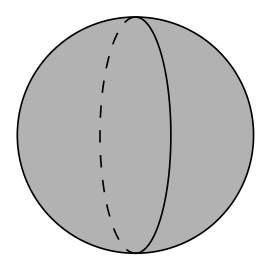
\includegraphics[width=0.10\textwidth]{p238_d1.png}\quad=\quad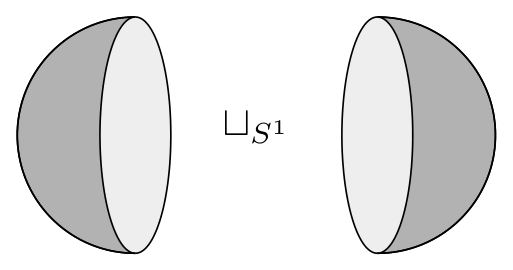
\includegraphics[width=0.22\textwidth]{p238_d2.png}
\end{equation}
（原文此处为示意图：$S^2$ 由两个半球沿 $S^1$ 粘合而成，右端标有 $\sqcup_{S^1}$），我们看到
\begin{equation}\tag{13.101}
\cZ(S^2)=\End\bigl(1_{\cZ(S^1)}\bigr),
\end{equation}
其中 $1_{\cZ(S^1)}$ 是平凡面缺陷。
% [Tutor Note: (13.100) 的图形在原书中为手绘示意（p.~237），此处保留原图。其含义是 $S^2$ 是 $S^1$ 上的“两个圆盘”的粘合，对应把线算子($S^2$) 写成面算子($S^1$) 的自同态；这正是 (13.101) 的内容。]

现在我们可以陈述：局部 Langlands 对应把 $G(K)$ 的光滑表示与 $\Loc_{G^\vee}(K)$ 联系起来/沿其谱分解。下面是一个具体的相应结果。

\begin{srcthm}{13 (Harris–Taylor, Henniart)}
对 $K$ 为局部域，$\mathrm{GL}_n(K)$ 的不可约光滑表示与 $K$ 上秩 $n$ 的 Galois 表示的同构类 $\Loc_{\mathrm{GL}_n}/\!\sim$ 双射。
\end{srcthm}
这是在说 $\Loc_{\mathrm{GL}_n}/\!\sim$ 在扮演某种 $\mathrm{GL}_n(K)$ 的 Pontrjagin 对偶的角色。但更一般的群呢？对一般群，人们已经（先由实验、现在已正式地）发现，$G(K)$ 的不可约表示映到 $\Loc_{G^\vee}$。即，这是自守到谱的方向：我们可以给一个不可约表示附上 Langlands 参数。
% [Tutor Note: 定理 13 中的“秩 $n$ Galois 表示”应理解为“$n$ 维 Galois 表示”（rank 指 $\mathrm{GL}_n$ 标准表示的维数，而非概形的秩）；且 $\Loc_{\mathrm{GL}_n}$ 此处指 $\Gal(K)$ 到 $\mathrm{GL}_n$ 的连续半单表示（带适当分歧条件）的栈，$\sim$ 表示同构。]

想法是：你应当能够给 $G(K)$ 的表示附上 Galois 表示，但这个映射不是一一的。这是在函数域设定中由 V.~Lafforgue–Genestier、在数域设定中由 Fargues–Scholze 给出的定理。这个映射的纤维称为 $L$-包。这些是 $L$-不可区分的表示，即 $L$-函数无法区分的表示。所以这不是一一对应，但这些包很小。

为什么我们有这种含糊性？其实我们应该在 $\Loc_{G^\vee}$ 上附一个层：一侧是 $G(K)$ 的表示，另一侧是 $\Loc_{G^\vee}$ 上某类层范畴。但 $\Loc_{G^\vee}$ 是栈，因为局部系统有自同构。所以即使一个层支撑在单个表示 $\rho:\Gal\to G^\vee$ 上，还有更多数据：$\Aut(\rho)$，即 $\rho$ 的中心化子，必须作用。于是我们得到
\begin{equation}\tag{13.102}
\Shv(\mathrm{pt}/Z(\rho))=\Rep(Z(\rho)).
\end{equation}
精细版本应说：$L$-包应构成这个中心化子 $Z(\rho)$ 的表示的一个子集，且这些表示在单位分支上平凡。即它是 $\pi_0(Z(\rho))$ 的表示。这告诉我们为什么应该期待这些包：我们先前把东西想得太过集合论了。

从这个图像我们得到一个全子范畴：
\begin{equation}\tag{13.103}
\Rep(G(K))\hookrightarrow \mathrm{Coh}(\Loc_{G^\vee}).
\end{equation}
这是局部 Langlands 对应的更精细版本。它在 $\mathrm{GL}_n$ 情形于 [BZCHN21] 中被证明。
% [Tutor Note: (13.102) 的 $\Shv(\mathrm{pt}/Z(\rho))$ 按定义就是 $Z(\rho)$-表示；之所以只剩下中心化子，是因为在栈上取点 $\mathrm{pt}\to\Loc$ 的纤维积要模掉稳定化子作用。这里 $Z(\rho)$ 可取为 $\rho$ 的 $\Gal$-中心化子（若 $\rho$ 不可约），其 $\pi_0$ 部分给出 $L$-包，连通部分给出无穷小特征。]

\begin{srcrem}{98}
这终于看起来像几何 Langlands 对应了。我们说局部域类似二维流形，而在几何 Langlands 中，谱侧是二维流形 $\Loc_{G^\vee}$ 上的某类凝聚层。但自守侧还不完全一样。
\end{srcrem}

如果我们看 $K=\C(\!(t)\!)$，那么这是一维流形的类比。所以我们该做高一层的事情，即我们在做局部几何 Langlands。于是我们考虑圈群
\begin{equation}\tag{13.104}
LG=G(K),
\end{equation}
并且不考察普通表示，而考察 $G(K)$-范畴。例如
\begin{equation}\tag{13.105}
G(K)\ \curvearrowright\ \Shv(G(K)/H)
\end{equation}
对任何子群 $H$。$LG=G(K)$-范畴的 2-范畴就是 TFT 附给一个圆周的东西：
\begin{equation}\tag{13.106}
\cA_G(S^1)=\Rep_{\mathbf{Cat}}(G(K)).
\end{equation}
于是我们可以把局部几何 Langlands 表述为：2-范畴 $\cA_G(S^1)$ 与 $\Loc_{G^\vee}(D^\times)$ 上的拟凝聚范畴层等同。如果我们改在 $\F_q(\!(t)\!)$ 上做这件事，那么它带有这个 Frobenius 作用；当我们取迹去范畴化时，就得到 $\F_q(\!(t)\!)$ 的局部 Langlands。

由此得到的局部 Langlands 版本实际上比我们上面表述的更好：我们得到等价而非全子范畴。我们先前对自守侧该放什么有点太天真了。有一个自然更大的范畴可供选择，它会与 $\mathrm{Coh}(\Loc_{G^\vee})$ 精确匹配。即 $\Rep(G(K))$ 太小了。下面的例子说明了这一点。

\begin{srcex}{93}
设 $G=T$。与其看所有表示，我们可以看非分歧表示。这只是一个 $T(K)$ 的表示，只不过现在我们取 $T(\cO)$ 的双陪集；但这是交换的（所以双陪集等同于单陪集），于是我们在考虑
\begin{equation}\tag{13.107}
\Gr_T=T(K)/T(\cO)\simeq\Lambda,
\end{equation}
其中 $\Lambda$ 是 $T$ 的特征格。于是
\begin{equation}\tag{13.108}
\Lambda\text{-}\mathbf{mod}\simeq\QC(T^\vee).
\end{equation}
\end{srcex}
% [Tutor Note: (13.107) 中仿射 Grassmann 簇 $T(K)/T(\cO)$ 的同构 $\simeq\Lambda$ 需固定一个均匀化子 $t$；作为格它是 $\Lambda$（余特征格，cocharacter lattice），而非特征格。原文称 $\Lambda$ 为 “character lattice”，此处照译但请注意：$T(K)/T(\cO)$ 自然地是余特征格。这一字之差会影响后续 $\Lambda$-mod 与 $\QC(T^\vee)$ 的对应方向。]
% [Tutor Note: (13.108) 中 $T^\vee$ 是环面，$\QC(T^\vee)$ 即 $\Lambda$-分次向量空间（取 $\Lambda$ 为 $T^\vee$ 的特征格时）。若按原文把 $\Lambda$ 当特征格，则 $\QC(T^\vee)$ 应是 $\Lambda^\vee=\Lambda$ 的分次，二者在环面情形恰好一致，故不影响结论。]

这看起来很好，但实际上这还不是全部。考虑非分歧局部系统：$\Loc^{\mathrm{unram}}_{T^\vee}$，即通过 Frobenius 分解的局部系统。于是其中之一由 Frobenius 在对偶群中的像，即 $T^\vee$ 的一个元素确定。但作为栈，它仍有自同构：
\begin{equation}\tag{13.109}
\Loc^{\mathrm{unram}}_{T^\vee}=T^\vee/T^\vee=T^\vee\times\mathrm{pt}/T^\vee.
\end{equation}
但当我们看它上面的层时，我们得到一个全子范畴：
\begin{equation}\tag{13.110}
\Lambda\text{-}\mathbf{mod}\simeq\QC(T^\vee)\hookrightarrow\QC(\Loc^{\mathrm{unram}}_{T^\vee}).
\end{equation}
即，我们先前只得到全子范畴（而非等价），是因为我们忽略了稳定化子。所以为了得到等价，我们需要这个额外因子：
\begin{equation}\tag{13.111}
\begin{array}{ccc}
\Lambda\text{-}\mathbf{mod} & \simeq & \QC(T^\vee)\\[4pt]
\downarrow & & \downarrow\\[4pt]
\Lambda\text{-}\mathbf{mod}\otimes\Rep(T) & \simeq & \QC\left(\Loc^{\mathrm{unram}}_{T^\vee}=\frac{T^\vee}{T^\vee}\right)
\end{array}
\end{equation}
% [Tutor Note: (13.111) 左下角的 $\Lambda\text{-}\mathbf{mod}\otimes\Rep(T)$ 中，$\Rep(T)$ 疑为 $\Rep(T^\vee)$ 之笔误：同一图右端是对偶环面的商栈 $T^\vee/T^\vee$，而 (13.112) 又把 $\Rep(T^\vee)$ 等同于 $\QC(\mathrm{pt}/T^\vee)$，所以“稳定化子修正”张量进来的应是对偶环面的表示范畴。原文照印 $\Rep(T)$，此处照译并标明。[译者按（无外部依据）]]
我们可以把这看作去范畴化的一次失败。当我们去范畴化时，对
\begin{equation}\tag{13.112}
\Rep(T^\vee)=\QC(\mathrm{pt}/T^\vee)
\end{equation}
有竖直/朴素的去范畴化和水平/聪明的去范畴化。竖直/朴素版本把这个范畴的 $\dim$ 当作普通范畴来取，得到
\begin{equation}\tag{13.113}
\dim\bigl(\Rep(T^\vee)\bigr)=\bigl(|\Rep(T^\vee)|,\bullet\bigr)=\cO(T^\vee).
\end{equation}
现在我们可以过渡到它上面的模：
\begin{equation}\tag{13.114}
\cO(T^\vee)\text{-}\mathbf{mod}=\QC(T^\vee).
\end{equation}
这是竖直/朴素的迹。

另一方面，我们可以取水平/聪明的版本，即把 $\Rep(T^\vee)$ 当作 $\otimes$-范畴来取 $\dim$；这更像代数的 Hochschild 同调，即最终会得到一个范畴。几何上，我们可以通过把 $\QC$ 与 $\dim$ 交换来计算它，即取 $\mathrm{pt}/T^\vee$ 的环路空间：
\begin{equation}\tag{13.115}
\QC\bigl(T^\vee/T^\vee=\mathcal{L}(\mathrm{pt}/T^\vee)\bigr).
\end{equation}
这是水平/聪明的迹。

注意这些并不一致：（竖直迹上的模）是水平迹的子范畴：
\begin{equation}\tag{13.116}
\QC(T^\vee)\hookrightarrow\QC(T^\vee/T^\vee).
\end{equation}
所以如果我们从几何 Langlands 出发，表述局部几何 Langlands，遵循我们一直遵循的同样规则，那么我们会试着去范畴化以弄清局部 Langlands 对应是什么。但我们可以做这两种迹。结论是：水平迹给你更好的东西。这已经出现在 V.~Lafforgue 的工作中，它引出了 excursion 算子的概念。这与先前的评论是同一回事：
\begin{equation}\tag{13.117}
\cO\left(\frac{G^\vee}{G^\vee}\right)\text{-}\mathbf{mod}\neq \QC\left(\frac{G^\vee}{G^\vee}\right).
\end{equation}
这个想法在 [AGK$^+$20b, AGK$^+$20a, AGK$^+$21] 中被精确化。
% [Tutor Note: (13.111) 的 2×2 图中第二行左端 $\Lambda$-mod$\otimes\Rep(T)$ 是把“稳定化子修正”张量进来；右端 $\QC(T^\vee/T^\vee)$ 正是水平迹（环路空间），它与 $\QC(T^\vee)$（竖直迹）的差别就是 (13.116) 的嵌入。(13.113) 中 $(\cdot,\bullet)$ 表示分次环（奇偶/度数），而 $\cO(T^\vee)$ 只看平凡分次，故竖直迹丢失了度数信息。]
% [Tutor Note: (13.117) 的不等号是本章最要紧的一句：$\cO(G^\vee/G^\vee)$-mod 是“朴素迹”，而 $\QC(G^\vee/G^\vee)$（即水平迹）才与自守侧匹配。这正是 V.~Lafforgue 的 excursion 算子与 AGK 的“谱分解”技术的关键差别，也是 (13.118) 要改用 $\IndCoh_{\mathrm{Nilp}}$ 的原因。]

\subsection{完整/范畴化局部 Langlands}\label{sec:13-6-4}

让我们回到算术设定（即 $K=\F_p(\!(t)\!)$、$\Q_p$ 等）。那么 $B$-侧是类似 $\QC(\Loc_{G^\vee})$ 的东西。然后我们希望它等价于某个包含 $\Rep(G(K))$ 作为全子范畴的范畴。答案是（拓扑）$\Bun_G$ 上的层，于是陈述的形状是\footnote{回忆 $\QC$ 其实应是 $\IndCoh_{\mathrm{Nilp}}$。}：
\begin{equation}\tag{13.118}
\Shv(\Bun_G)\simeq\QC(\Loc_{G^\vee}).
\end{equation}
所以我们只需弄清 $\Bun_G$ 是什么。我们知道
\begin{equation}\tag{13.119}
\Rep(G(K))=\Shv(\mathrm{pt}/G(K)),
\end{equation}
即它是某个空间中平凡丛轨迹上的层。所以会有一个更大的空间叫 $\Bun_G$，如果只看平凡丛，它的自同构是 $G(K)$。于是 $G(K)$ 的表示会作为生活在平凡丛轨迹上的层出现。但我们缺了这个空间的其余部分，而这就是几何 Langlands 观点所提议的。

这个 $\Bun_G$ 有两个版本。在函数域上更容易说：
\begin{equation}\tag{13.120}
\Bun_G=G(K)/_F G(K),
\end{equation}
其中 $/_F$ 表示模掉 Frobenius 扭共轭，即模掉作用
\begin{equation}\tag{13.121}
h*g=hgFh^{-1}.
\end{equation}
这来自顺着我们的鼻子走：如果我们想 $\Bun_G(D^\times)=\mathrm{pt}/G(K)$，然后求 Frobenius 的不动点。同构类的集合
\begin{equation}\tag{13.122}
G(K)/_FG(K)
\end{equation}
由所谓的 Kottwitz $G$-同晶（isocrystal）构成。

这预期大致等价于 Fargues–Scholze 的某个版本。他们研究某条特定曲线——称为 Fargues–Fontaine 曲线——上 $\Bun_G$ 的层。所以这真的是把“局部 Langlands 应该是某条特定曲线上的几何 Langlands”这个想法放在心上。即局部域 $K$ 应对应于某条曲线。在 $K=\Q_p$ 的情形，这条曲线大致是
\begin{equation}\tag{13.123}
\Spec\Q_p/\Z,
\end{equation}
其中 $\Z$ 通过 Frobenius 作用。我们可以把它想成某种模 Frobenius 的穿孔圆盘。要正确地说出这件事，你需要整套完美胚（perfectoid）机器。
% [Tutor Note: (13.118) 的脚注不可略过：光滑/有限型假设下 $\QC$ 与 $\IndCoh$ 的差别在 $\Bun_G$ 这类非有限型、非光滑对象上是本质的；正确陈述用 $\IndCoh_{\mathrm{Nilp}}(\Loc_{G^\vee})$。(13.120) 的 Kottwitz 同晶集合并不能直接给出 $\Bun_G$ 的几何结构，取 $G(K)/_FG(K)$ 作为“空间”只是对同构类的粗描述。]
% [Tutor Note: (13.121) 中 $F$ 是 Frobenius 自同构，$h*g=hgFh^{-1}$ 中的 $gF$ 表示 $\sigma$-线性作用；把它读作“$h g \sigma(h)^{-1}$”更不会出错。$\Bun_G=G(K)/_FG(K)$ 只对函数域（或完美胚意义下的 $\Q_p$）有意义，见 Fargues–Fontaine 曲线。]

\begin{flushright}\small 第 33 讲；2021 年 6 月 24 日\end{flushright}
